\documentclass{mcmthesis}
\mcmsetup{CTeX = true,   % 䜿甚 CTeX 套装时讟眮䞺 true
        tcn = 83451, problem = C,
        sheet = true, titleinsheet = true, keywordsinsheet = true,
        titlepage = false, abstract = false}
\usepackage{palatino}
\usepackage{graphicx}
\title{The \LaTeX{} Template for MCM Version \MCMversion}
\author{\small Team \# 83451}
\date{\today}
\begin{document}

\begin{abstract}

This is a try of our paper. Mainly test how to insert a beautiful table and a nice picture of our work. In the end, we tried how to show a nice Reference.

\begin{keywords}
  Try; Table; Picture; Reference
\end{keywords}
\end{abstract}
\maketitle

\tableofcontents
\newpage

\section{Introduction}

    Have a try before doing something is very important these days. Since the tasks are getting harder and harder than old days.So we need to get into this kind of trend.

    As for this paper. This is a try of our paper. Mainly test how to insert a beautiful table and a nice picture of our work. In the end, we tried how to show a nice Reference.\cite{crocker1986introduction}

\section{Assumptions}

    To simplify the real life situation, we will accept the following assumptions while we construct our models.

    \begin{itemize}

      \item We have a plenty of time for having a try.
      \item If we have a try, we can get to work better at the real contest.

    \end{itemize}

\section{Notations}

    \begin{table}[h]
      \centering
        \begin{tabular}{|c|c|c|}

          \hline Notations & Definition & Unit \\
          \hline $T$ & The totle time for us to have a try & $s$ \\
          \hline $t_{min}$ & The minimize try time & $s$ \\
          \hline

        \end{tabular}
        \caption{Notations}
    		\label{tab:Notations}
    \end{table}

\section{Models}
  \subsection{Existing Model}
    The basic model at now we are using is based on the ...

  \subsection{Updating Model}
    We then update out model to a more efficient one ...

  \subsection{The Brand-new Model}
    To satistify the ...
    \\
    \begin{figure}[ht]

      \centering
      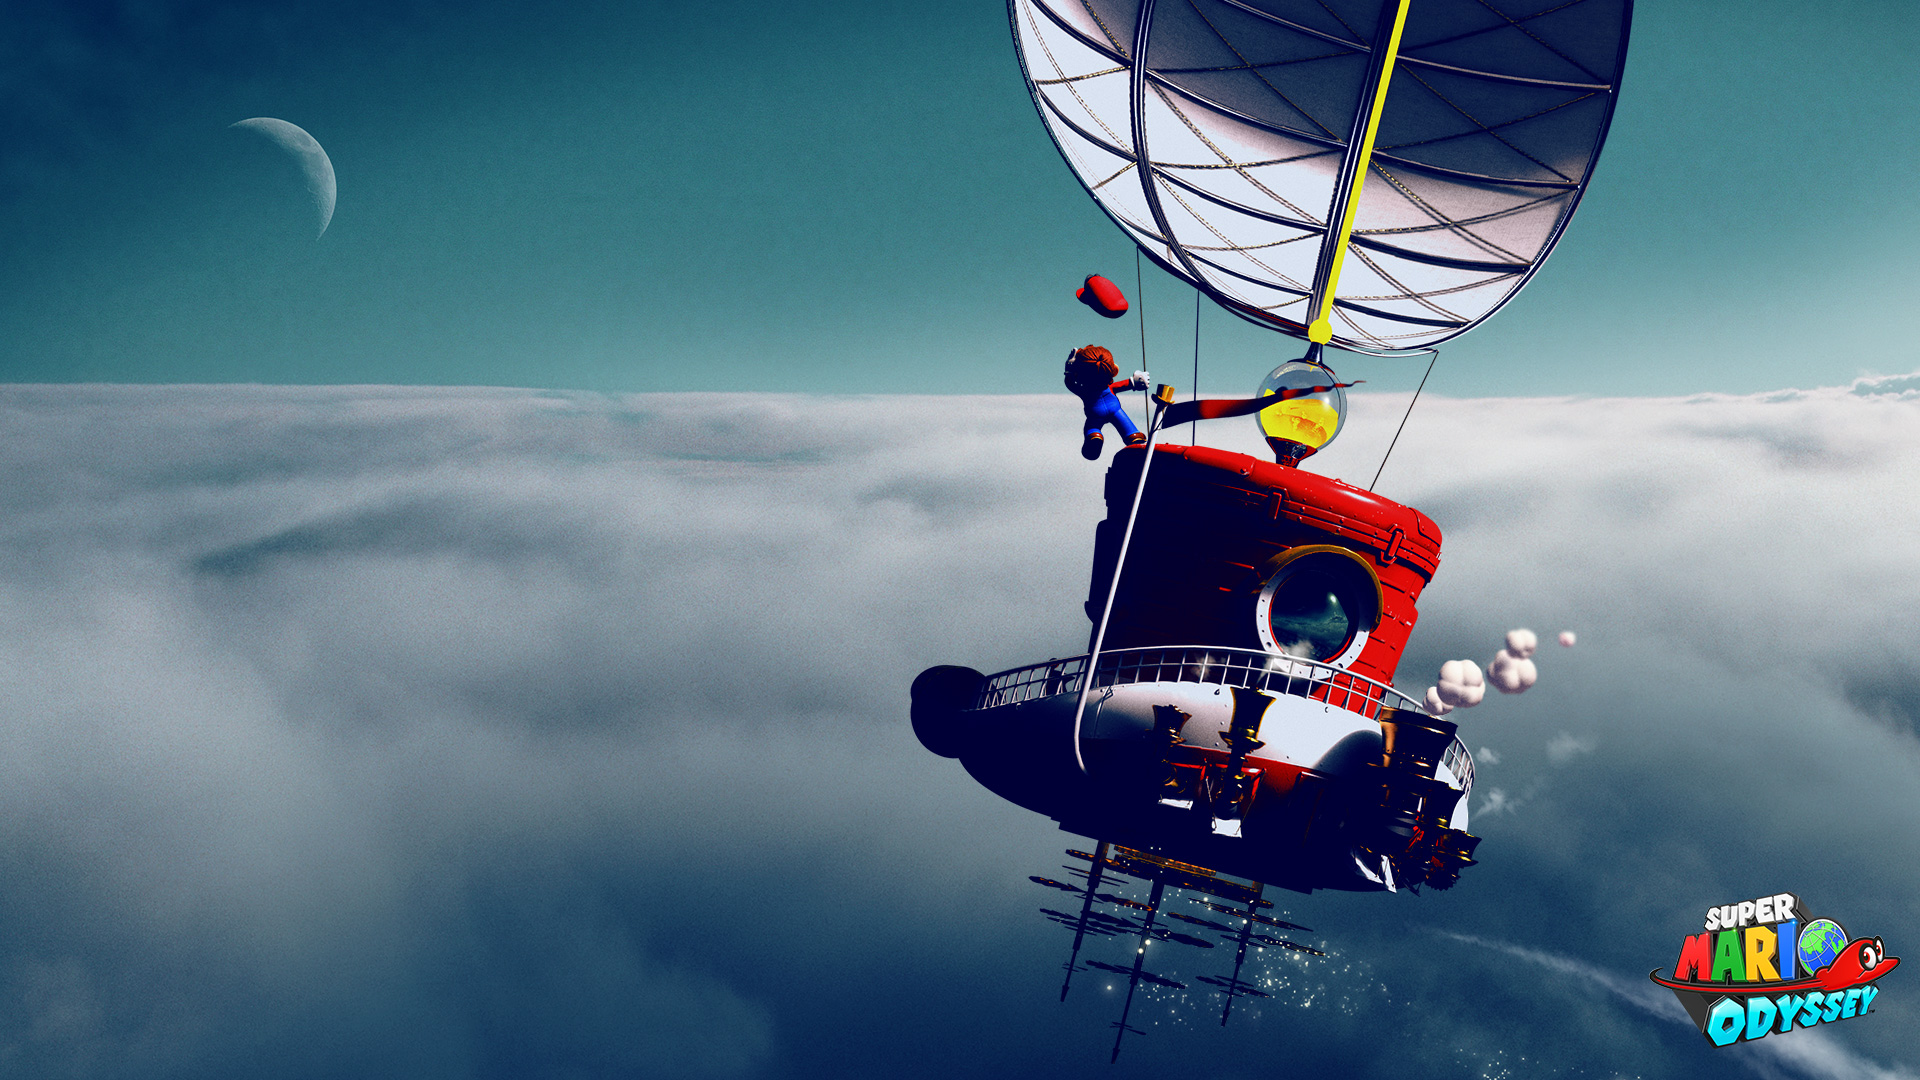
\includegraphics[scale=0.22]{pictures}
      \caption{Mario~!}
      \label{fig:label}

    \end{figure}


\section{Analysis and Results}

blablablablablabla...

\section{Sensitive Test}

rua!~~~~

\section{Strengths and Weaknesses}
  \subsection{Strengths}
    Huuuuuuge!
  \subsection{Weaknesses}
    Rueeeee
  \subsection{Possible Modifications}
    mmmmmmm


\section{Conclusion}

Conclusion is here~!


\newpage
% \begin{thebibliography}{99}
%
%     \bibitem{1} D.~E. KNUTH   The \TeX{}book  the American
%     Mathematical Society and Addison-Wesley
%     Publishing Company , 1984-1986.
%     \bibitem{2}Lamport, Leslie,  \LaTeX{}: `` A Document Preparation System '',
%     Addison-Wesley Publishing Company, 1986.
%     \bibitem{3}\url{http://www.latexstudio.net/}
%     \bibitem{4}\url{http://www.chinatex.org/}
%
% \end{thebibliography}

\bibliographystyle{plain}
\bibliography{new_t}

\newpage
\begin{appendices}

  \section{First appendix}

    Here are simulation programmes we used in our model as follow.\\

    \textbf{\textcolor[rgb]{0.98,0.00,0.00}{Input Matlab source:}}


  \section{Second appendix}

    some more text \textcolor[rgb]{0.98,0.00,0.00}{\textbf{Input Python source:}}


\end{appendices}



\end{document}
